\documentclass[10pt]{article}

% Page geometry - single page, tight margins matching the template
\usepackage[a4paper, top=1.8cm, bottom=1.8cm, left=1.8cm, right=1.8cm]{geometry}

% Font - Helvetica (similar to Calibri, pdflatex compatible)
\usepackage[scaled]{helvet}
\renewcommand\familydefault{\sfdefault}
\usepackage[T1]{fontenc}

% Single spacing
\usepackage{setspace}
\singlespacing

% Graphics for the system diagram
\usepackage{graphicx}
\usepackage{caption}

% Two-column layout for abstract/body sections
\usepackage{multicol}

% Remove page numbers
\pagestyle{empty}

% Hyperlinks (optional, clean)
\usepackage[hidelinks]{hyperref}

% Compact lists
\usepackage{enumitem}
\setlist{nosep, leftmargin=*, topsep=0pt}

% Section formatting - bold, no numbering, tight spacing
\usepackage{titlesec}
\titleformat{\section}{\bfseries\normalsize}{}{0em}{}
\titlespacing{\section}{0pt}{6pt}{3pt}

% Reduce paragraph spacing
\setlength{\parindent}{0pt}
\setlength{\parskip}{4pt}

\begin{document}

% ============================================================
% TITLE BLOCK
% ============================================================
\begin{center}
{\large\bfseries KrishokChat: A Safety-First Agentic Agricultural Advisory System\\for Bangladeshi Smallholder Farmers}\\[4pt]
{\normalsize Field-Collected Crop Disease and Soil Moisture Datasets with a Four-Stage Verified Bengali AI Pipeline}
\end{center}

\vspace{4pt}

\begin{multicols}{2}

% ============================================================
% ABSTRACT [100 words]
% ============================================================
\section*{ABSTRACT}

KrishokChat is an end-to-end agricultural advisory system built for Bengali-speaking smallholder farmers in Bangladesh. Farmers submit crop questions in Bengali or upload photographs of diseased leaves, and the system returns source-cited treatment guidance through a four-stage agentic pipeline that classifies safety risk, retrieves from government-sourced knowledge, generates grounded answers, and verifies chemical dosage claims before they reach the farmer. The system covers 37 disease classes across five major crop families. Two original field-collected datasets accompany the platform: a 722-image tensiometer-labeled soil moisture dataset from Pabna District and a 1,000-query farmer benchmark from structured interviews. Two research manuscripts are under peer review.

% ============================================================
% METHOD WITH SYSTEM DIAGRAM [100 words]
% ============================================================
\section*{Method with System Diagram}

The system operates as a layered agentic pipeline rather than a single model call. A farmer's query first passes through a safety classifier with six risk categories (safe agriculture, banned chemicals, self-harm, off-topic, prompt injection, low confidence). Terminal categories receive an immediate referral to the Krishi Call Center (16123) without triggering any retrieval. Safe queries proceed to a hybrid retrieval engine over 2,120 knowledge nodes extracted from 2,946 government publications. Retrieved passages feed a fine-tuned language model that streams Bengali answers, followed by a dosage verification agent that flags ungrounded chemical claims against source evidence.

% Insert your generated system diagram here
% Replace 'figure.png' with your actual filename
\begin{center}
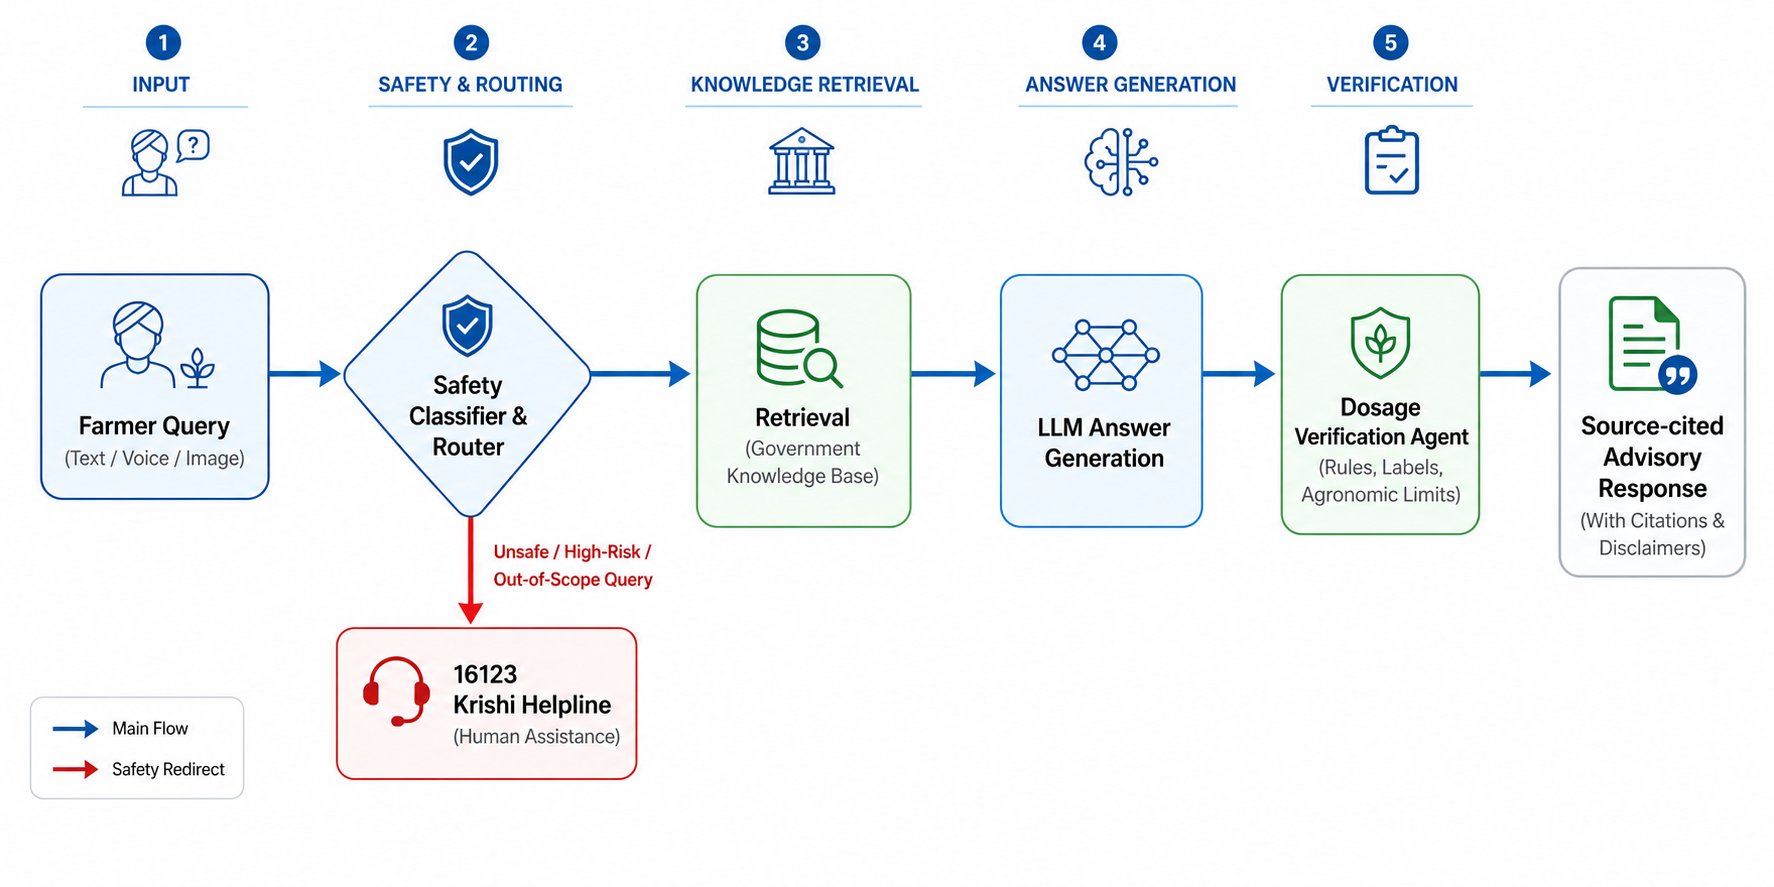
\includegraphics[width=\columnwidth]{figure.png}
\captionof{figure}{KrishokChat four-stage agentic advisory pipeline with vision-based crop disease routing and safety-first query classification.}
\end{center}

% ============================================================
% NOVELTY [50 words]
% ============================================================
\section*{Novelty of Project}

Existing agricultural chatbots (Farmer.Chat, KrishokBondhu) lack pre-retrieval safety classification, structured dosage verification, and field-collected Bengali datasets in one integrated platform. KrishokChat is the first system that enforces a four-stage safety-verified agentic pipeline for Bengali agricultural advice, backed by an 85,979-instance provenance-traced benchmark and original field data from Bangladeshi farming communities.

% ============================================================
% IMPACT [50 words]
% ============================================================
\section*{Impact on Society/Environment}

Incorrect pesticide dosage advice causes crop failure, health hazards, and soil contamination across rural Bangladesh. By verifying every chemical recommendation against government-approved sources and refusing unsafe queries with helpline referrals, KrishokChat directly reduces the risk of pesticide misuse among the 47 million farming households who currently lack access to reliable Bengali-language advisory services.

% ============================================================
% BUSINESS MODEL [100 words]
% ============================================================
\section*{Business Model / Feasibility / Scalability}

KrishokChat runs entirely on a single machine without cloud dependencies, making deployment feasible in low-connectivity rural settings. The initial rollout targets agricultural extension offices and farmer cooperatives through a freemium model: basic crop advisory and disease diagnosis are free, while premium features like personalized seasonal planning and bulk farm management tools generate subscription revenue. Partnerships with government bodies (DAE, BARC) and agricultural input companies provide institutional licensing and sponsored advisory content. The system's modular architecture allows adding new crops, diseases, and regional dialects without rebuilding the core pipeline. The publicly released datasets and benchmark enable third-party validation and ecosystem growth.


% ============================================================
% CONCLUSION [50 words]
% ============================================================
\section*{Conclusion}

The safety-aware advisory pipeline, crop disease diagnosis across five families, Bengali chat interface with real-time streaming, and the soil moisture field dataset are fully implemented and functional. Remaining work within the final week includes soil moisture regression model training, additional dialect coverage testing, and preparation of the recorded demonstration for the final showcase.

\end{multicols}

\end{document}
